\section{แนวคิดและวิธีการดำเนินงาน}

ในการดำเนินงานนั้น

\clearpage
% \begin{figure}[ht!]
%     \centering
%     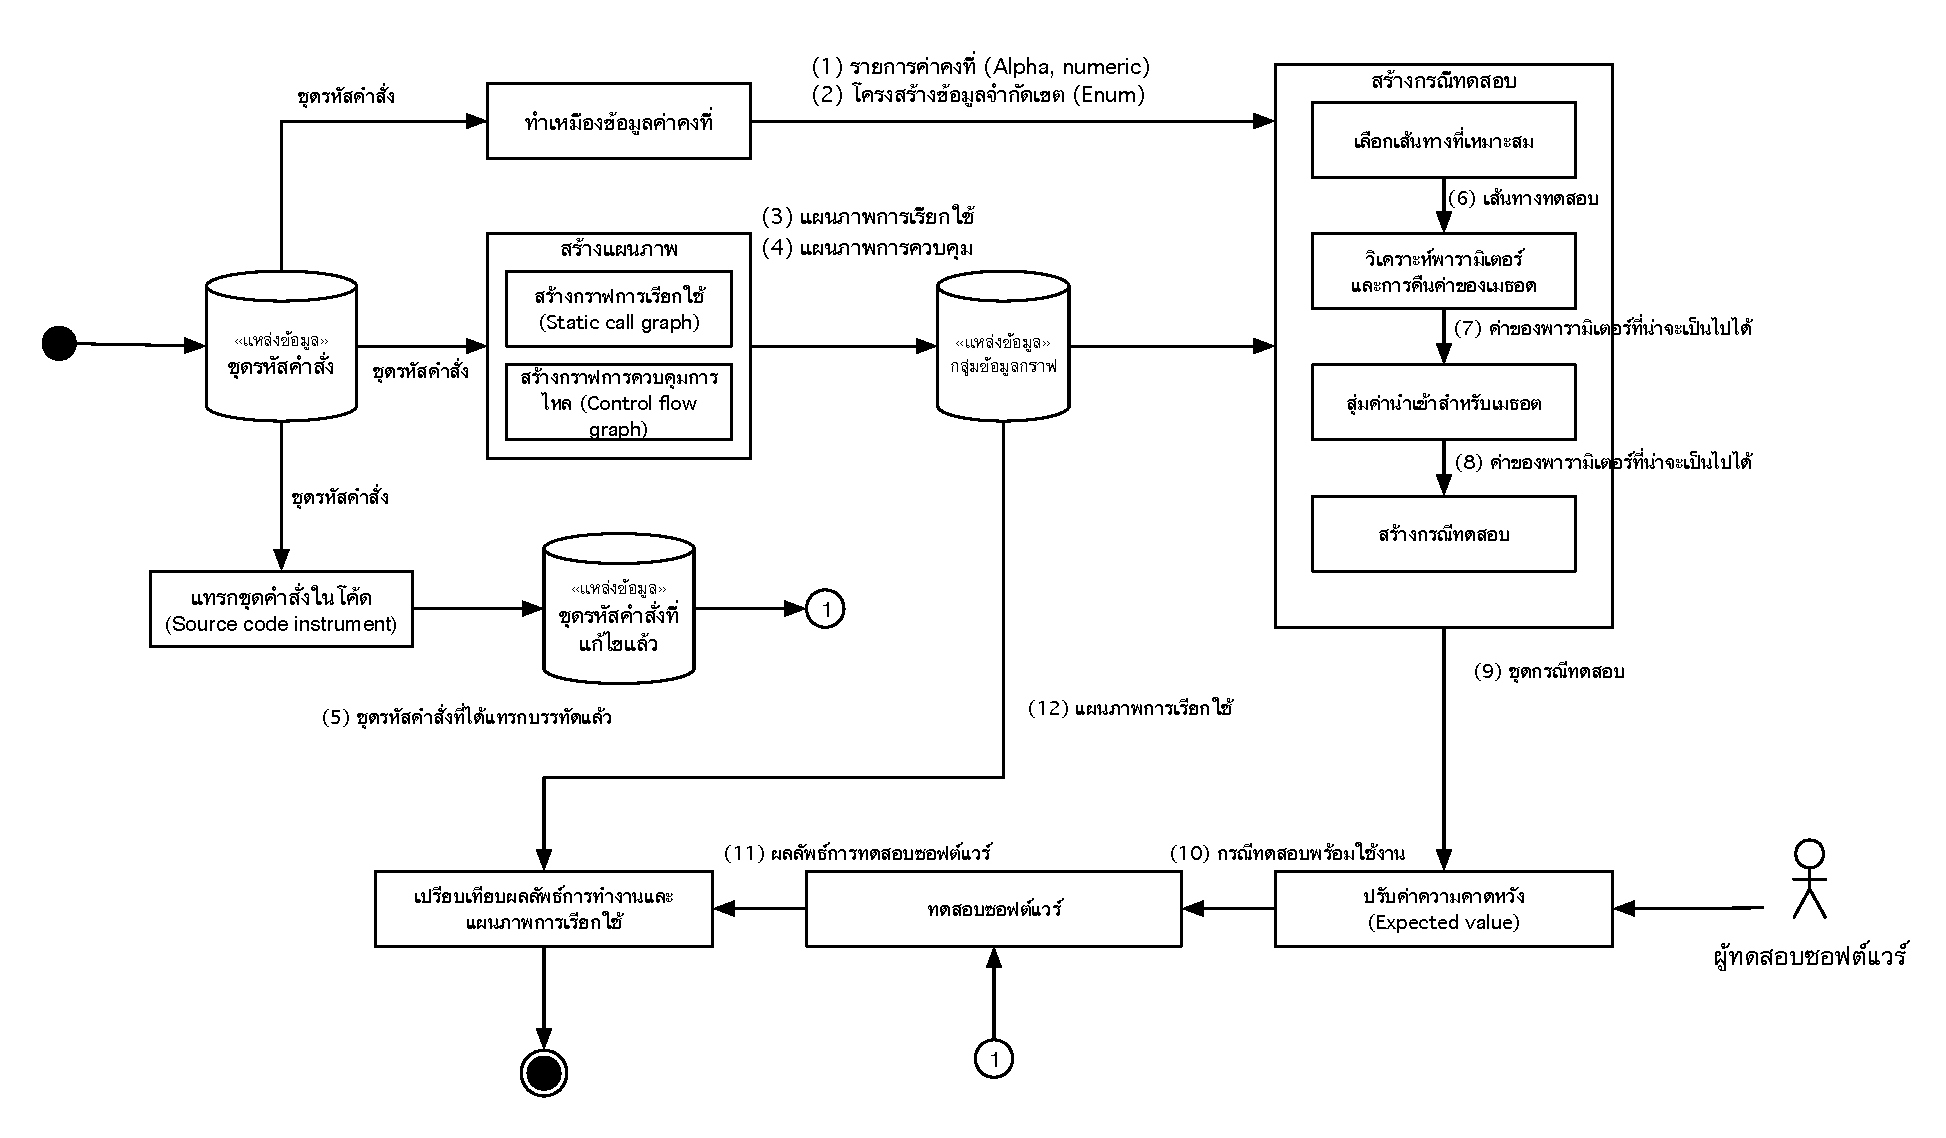
\includegraphics[height=\textwidth]{methodology-overview}
%     \caption{ภาพรวมการดำเนินงานวิจัย}
%     \label{fig:methodologyoverview}
% \end{figure}

\subsection{ภาพรวมงานวิจัย}
\begin{landscape}
    \begin{figure}[ht!]
        \centering
        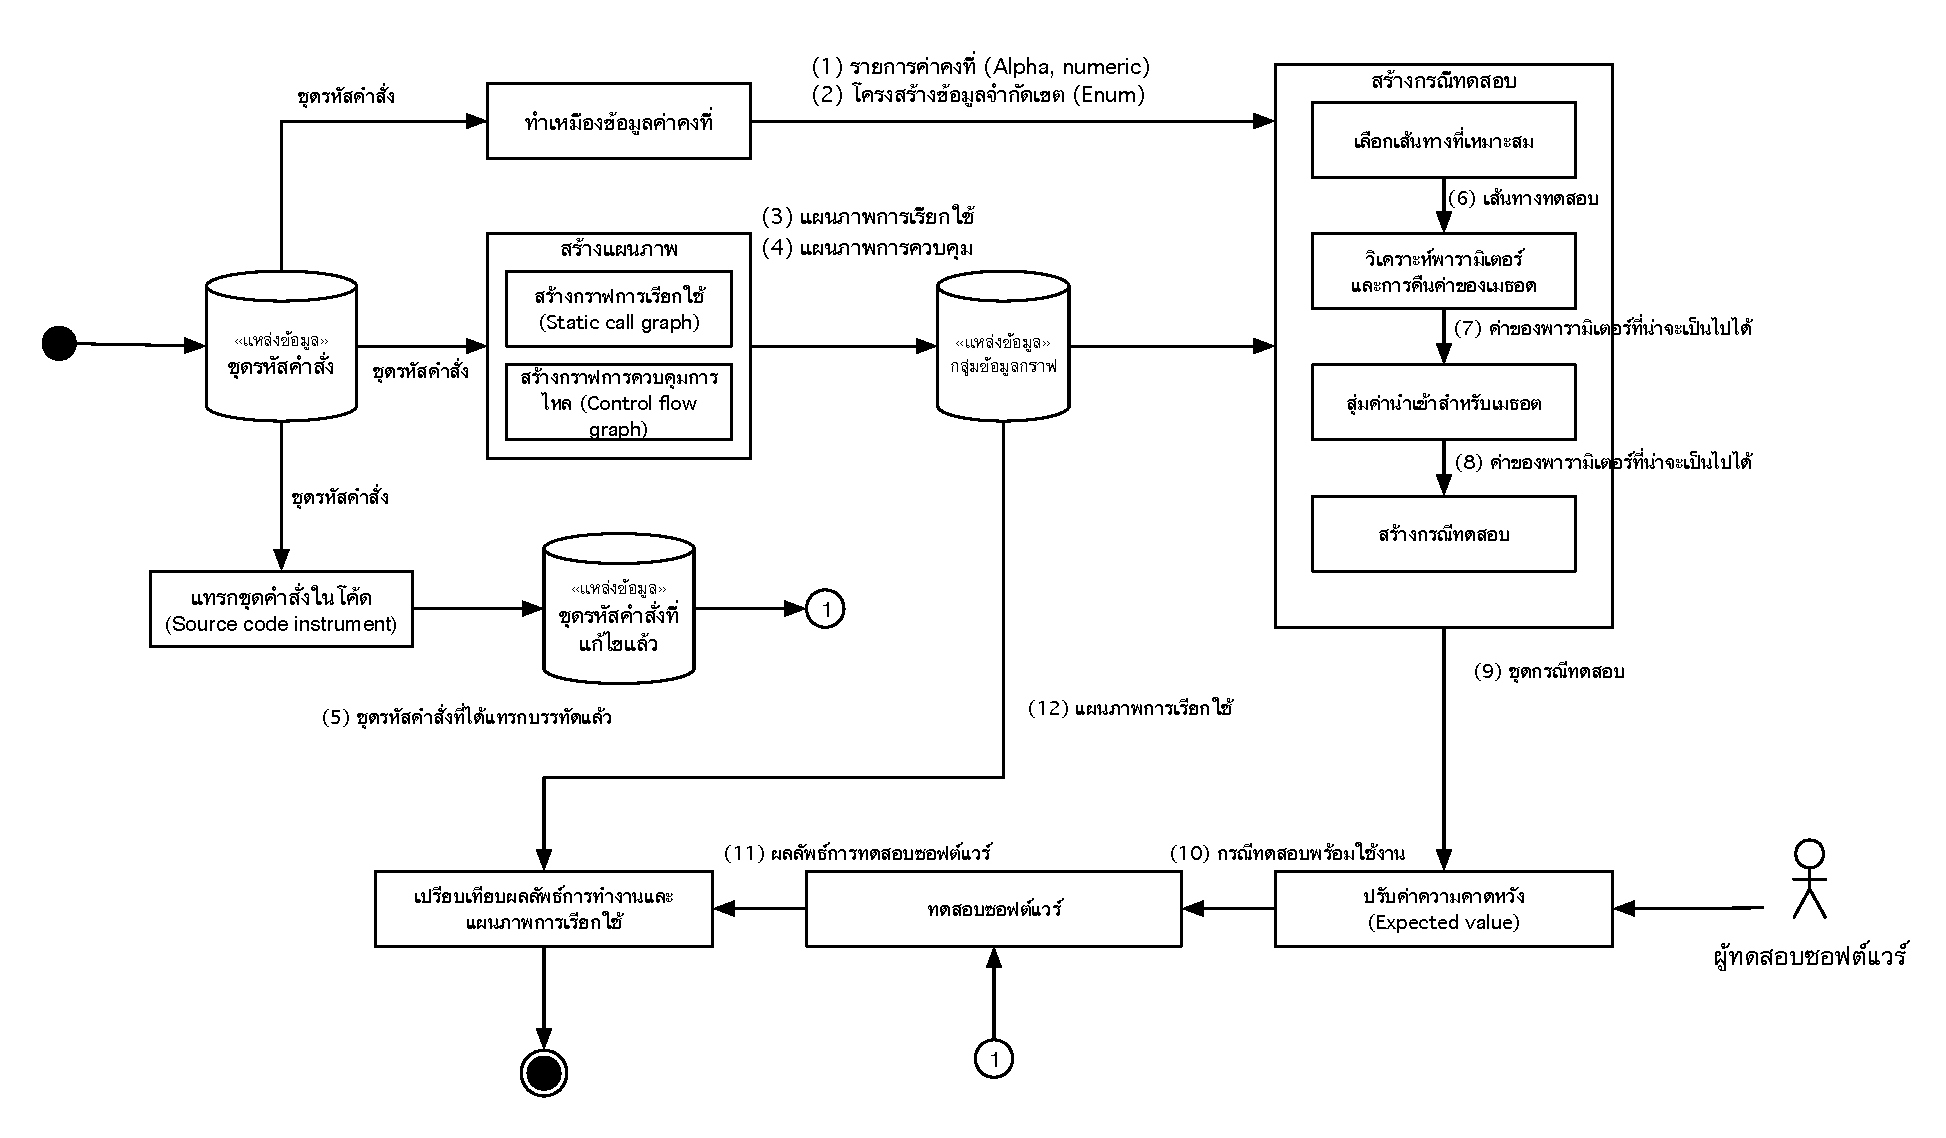
\includegraphics[height=0.9\textwidth]{methodology-overview}
        \caption{ภาพรวมการดำเนินงานวิจัย}
        \label{fig:methodologyoverview}
    \end{figure}
\end{landscape}

\subsection{กระบวนการทำงาน}
\begin{figure}[ht!]
    \centering
    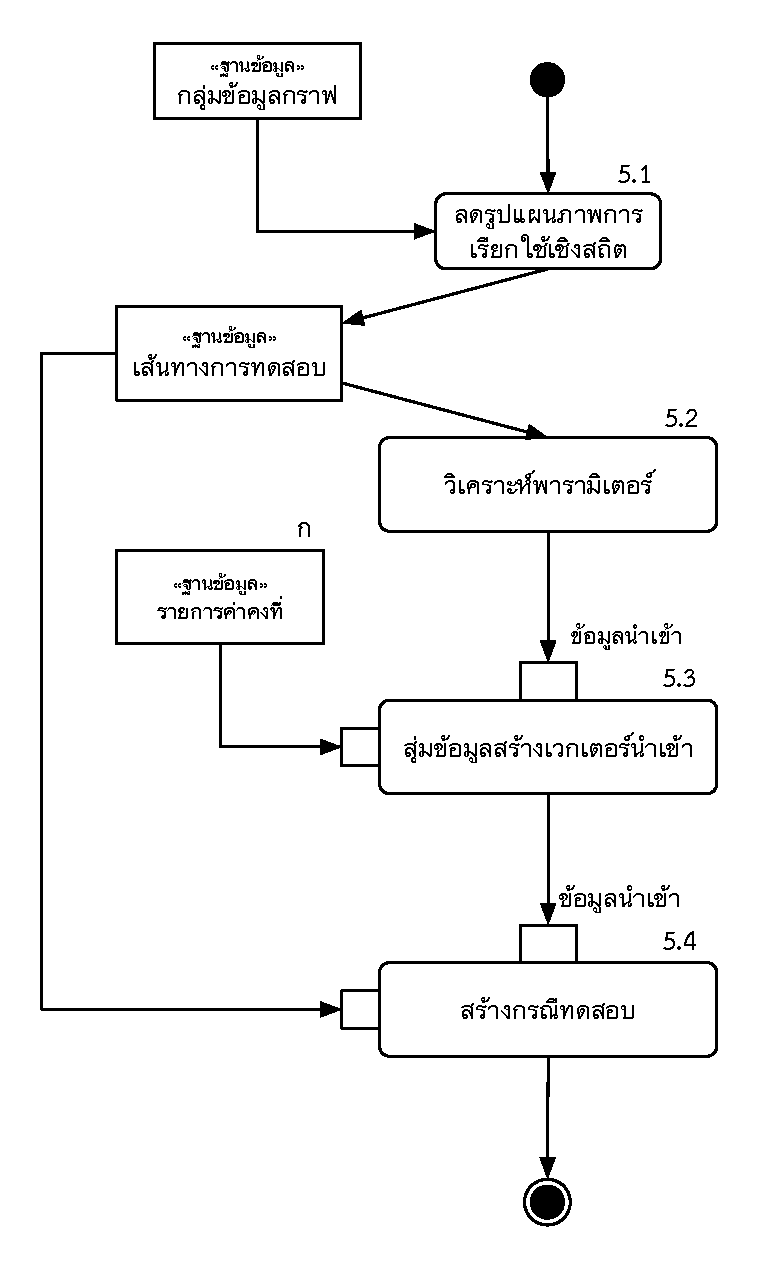
\includegraphics[width=0.6\textwidth]{methodology-activities-test-case-gen}
    \caption{ขั้นตอนการสร้างกรณีทดสอบจากข้อมูล}
    \label{fig:methodologyactivity}
\end{figure}
